\documentclass{article}

% packages
\usepackage[english]{babel}
\usepackage[utf8]{inputenc}
\usepackage{amsmath}
%\usepackage{amssymb}
%\usepackage{amsthm}
\usepackage{braket}
\usepackage{graphicx}
%\usepackage{bbm}
%\usepackage{multirow}
\usepackage{tikz}
\usetikzlibrary{positioning}
\usetikzlibrary{shapes.arrows}
\usepackage{color}
%\usepackage[colorinlistoftodos]{todonotes}
%\usepackage[absolute,overlay]{textpos}
%\usepackage{hyperref} % Should be last package imported
\usepackage{fullpage}

%%%%%%%%%%%%%%%%%%%%%%%%%%%%%%%%%%%%%%%%%%%%%%%%%
%%% SHORTCUTS %%%

%\newcommand{\pagehline}{\\\specialrule{.01pt}{0pt}{5pt}}
\newcommand{\pagehline}{\noindent\rule{\textwidth}{0.2pt}}

\newcommand{\paren}[1]{\left( #1 \right)}
\newcommand{\expectation}[1]{\left< #1 \right>}
\newcommand{\brac}[1]{\left[ #1 \right]}
\newcommand{\zerodel}{.\kern-\nulldelimiterspace}
\newcommand{\abs}[1]{\left\vert #1 \right\vert}
\newcommand{\wt}[1]{\widetilde{#1}}

\newcommand{\vecE}{\mathbf{E}}
\newcommand{\vecB}{\mathbf{B}}
\newcommand{\kvec}{\mathbf{k}}
\newcommand{\xvec}{\mathbf{x}}
\newcommand{\rvec}{\mathbf{r}}
\newcommand{\bvec}{\mathbf{b}}
\newcommand{\Rvec}{\mathbf{R}}
\newcommand{\zbar}{\overline{z}}
\newcommand{\curl}{\nabla\times}
\renewcommand{\div}{\nabla\cdot}

\DeclareMathOperator{\Lagr}{\mathcal{L}}
\DeclareMathOperator{\Ham}{\mathcal{H}}
\DeclareMathOperator{\tr}{tr}

\newcommand{\lucas}[1]{\textcolor{blue}{\bf [LKW #1]}} % Lucas comment


\title{\vspace{-3em} Fitting a band structure model for silicon\vspace{-2em}}
\date{}

\begin{document}
\maketitle

\section{Goals}

\begin{enumerate}
\item Calculate the band gap $E_g$ of silicon
\item Compute silicon bands near the Fermi level 
\end{enumerate}

\section{Motivation}

Electronic materials are commonly understood through the band structure model, in which non-interacting particles each occupy a particular quantum state in the material. 
Electronic excitations are understood as electrons moving between states with different energies.
Within the band structure model, the total electronic energy $E$ is given by

\begin{equation}\label{eq:bsm}
E = \sum_i \epsilon_i n_i,
\end{equation}

where $\epsilon_i$ and $n_i$ are the energy and occupation of state $i$.  
In the ground state, all orbitals with energies below the Fermi energy $E_F$ are fully occupied, and all orbitals with higher energies are empty. 
Although this model does not account for electron correlations, it gives a useful description for electronic and optical properties of many materials.

As a single-particle description, the band structure can be computed using \emph{ab initio} mean-field methods, which give good qualitative predictions but sometimes have quantitative errors, for example DFT often underestimates the band gap.
More accurate corrections to the electronic energies have been obtained by taking many-body correlation effects into account.
While perturbation theory methods have been used to this end, so far QMC has not been used to calculate band structures.

We demonstrate a method to compute band structure from QMC and apply it to silicon, which has been well understood both experimentally and theoretically.

\section{Band gap model}

To demonstrate the idea, we construct a simple model to compute the energy of the transition from the valence band at $\Gamma$ to the conduction band at $X$ (the lowest transition occuring in a conventional cell with periodic boundary conditions).

We only need to consider this excitation from the ground state, and can leave all other states' occupations unchanged.
This simplifies Eq \ref{eq:bsm} to

\begin{equation}
E = E_0^{\rm filled} + \epsilon_v n_v + \epsilon_c n_c,
\end{equation}

where $E_0^{\rm filled}$ is a constant (accounting for the energy of all the fully occupied valence states), $\epsilon_v$ and $n_v$ are the energies and occupations of the state at the VBM, and the subscript $c$ refers to the CBM.
Since the total number of electrons is conserved ($n_v + n_c = C$ is constant), we can rewrite the model as

\begin{equation}\label{eq:bandgapmodel}
E = E_0 + E_g n_c,
\end{equation}

where $E_0$ is the energy of the ground state (all states below $E_F$ occupied), and $E_g = \epsilon_c - \epsilon_v$ is the band gap.
The CBM of silicon is at the $X$ point in the Brillouin Zone, which has two degenerate bands in DFT, and is equivalent to points in the $y$ and $z$ directions by symmetry, for a total of six degenerate states at the CBM.
We therefore use $n_c$ to denote the sum of the occupations over all six of these states.

In order to define the model in the context of fitting to QMC, we make two assumptions:

\begin{enumerate}
\item DFT gives qualitatively correct quasiparticle degeneracies and gaps at $\Gamma$ and $X$.
\item The Kohn-Sham orbitals are the right orbitals to describe the quasiparticles.
This means two things: 
(a) using these to generate trial functions for QMC will allow us to sample the lowest energy excitations; 
(b) only these orbitals will show varying occupation in the many-body calculation.
\end{enumerate}

\section{Mean field calculation}

%We simulate the conventional unit cell (diamond structure) with 8 Si atoms (16 up electrons, 16 down).
DFT was run in PySCF using the PBE xc-functional and BFD pseudopotentials.
The BFD basis set was used with exponents less than $0.1$ removed.
Kohn-Sham orbitals were computed at the gamma point (which includes the X point of the primitive cell).
There are 16 occupied orbitals in the lowest energy mean-field wave function.


\section {Sampling states}

To fit the model in Eq \ref{eq:bandgapmodel}, we compute the energy $E$ and CB occupation $n_c$ for many sample wave functions.
DMC calculations require the fixed-node approximation, which finds the lowest energy state consistent with the nodal structure of the trial function.
This works to our advantage when fitting low-energy models: we can sample different excitations by selecting trial functions with different nodes. 
The trial functions are linear combinations of Slater determinants,

\begin{equation}
\Psi^S = \sum_i c_i D_i,
\end{equation}

where each Slater determinant $D_i$ is chosen by promoting electron(s) from an occupied orbital to an empty orbital.


For the band gap model, we choose combinations of determinants 


\subsection{DFT states}
To describe the low energy degrees of freedom, we choose determinants corresponding to low energy mean-field excitations.
The DFT orbital energies are shown in Fig \ref{fig:dft_energies}.

\begin{figure}[h]
\begin{center}
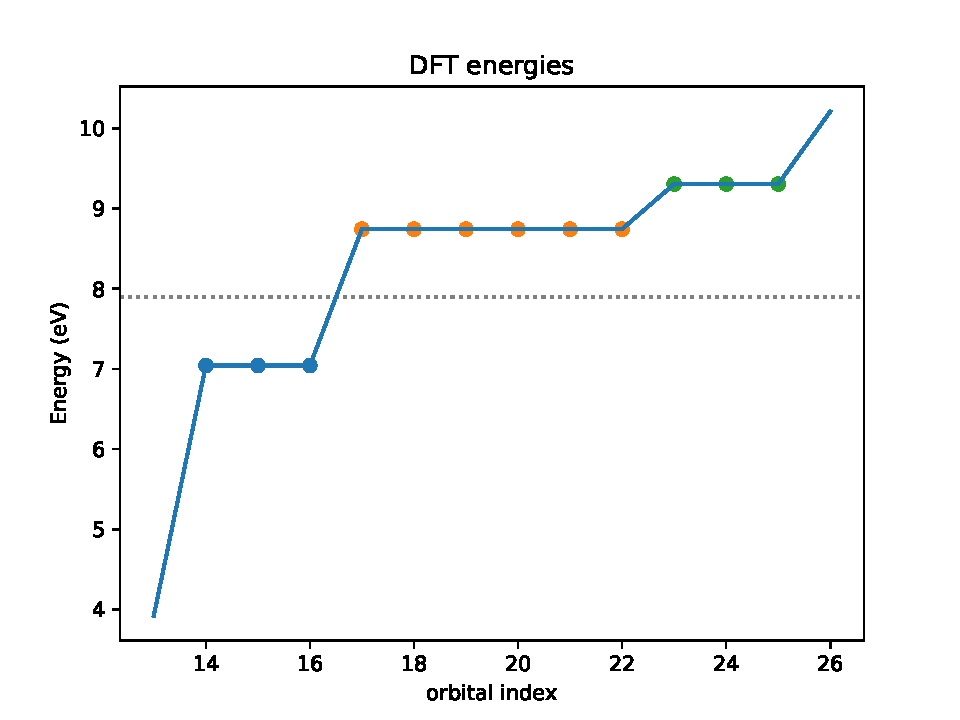
\includegraphics{images/dft_energies_k888.pdf}
\label{fig:dft_energies}
\caption{DFT orbital (single particle) energies. 
Dots are the orbitals used to generate excitations. 
Dotted gray line is the Fermi energy.}
\end{center}
\end{figure}

The states sampled for the model are combinations of Slater determinants multiplied by a Jastrow factor.
The Slater determinant part is defined as

\begin{equation}
\Psi^S = \sum_i c_i D_i,
\end{equation}

where each Slater determinant $D_i$ is chosen by promoting electron(s) from an occupied orbital to an empty orbital.
The weights $c_i$ are normalized, so the number of tunable parameters is one less than the number of determinants.

The final wave function has the form

\begin{equation}
\Psi = \Psi^S \Psi^J,
\end{equation}

where the Jastrow factor $\Psi^J$ is optimized to minimize the energy given the nodal structure of $\Psi^S$.
This is done to project out the components of the wave function not in the desired low-energy subspace.

\subsection{Choosing excitations}

\begin{figure}[h!]
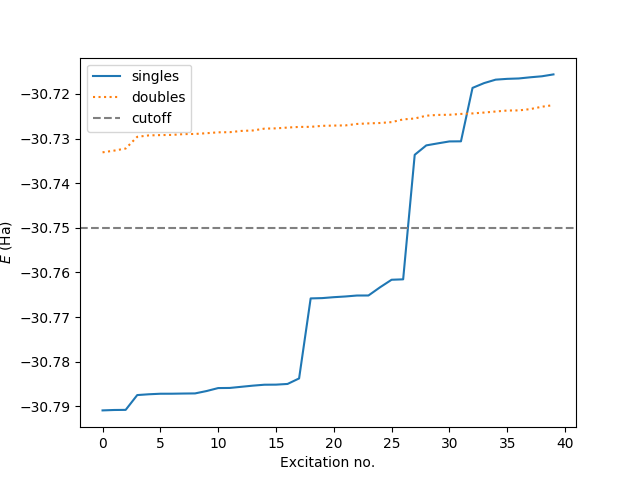
\includegraphics[width=0.5\textwidth]{images/determinant_mf_energies.png}
\label{fig:energy_cutoff}
%TODO update old data!
\caption{\textcolor{red}{\bf !!OLD DATA!!} Mean-field DFT total energies for singles and doubles excitations.
The dashed line shows the cutoff chosen for the samples used in this calculation.}
\end{figure}

To fit a ``low energy'' model, it is ideal to choose states below an energy gap so that the states are well described by the low energy subspace of the Hilbert space.
(If there is no gap, the states may have components not included in the low energy space, introducing energy variance that is not relevant to the model.)
We choose an energy cutoff in the gap shown in Fig \ref{fig:energy_cutoff}, which only includes singles excitations.

\subsection{Wave function samples}

The model we consider here assigns energies to the molecular orbitals,

\begin{equation}
E = \epsilon_0 + \sum_i \epsilon_i n_i,
\end{equation}

where $i$ indexes a set of molecular orbitals, and the orbital energies $\epsilon_i$ are model paramaters that are fit to the QMC data.
In this set of samples, a total of 12 orbitals have varying occupation (three valence, nine conduction, Fig \ref{fig:descriptors}).
Since the total number of electrons is constant, there are only 11 degrees of freedom in the orbital occupations.

\begin{figure}[h!]
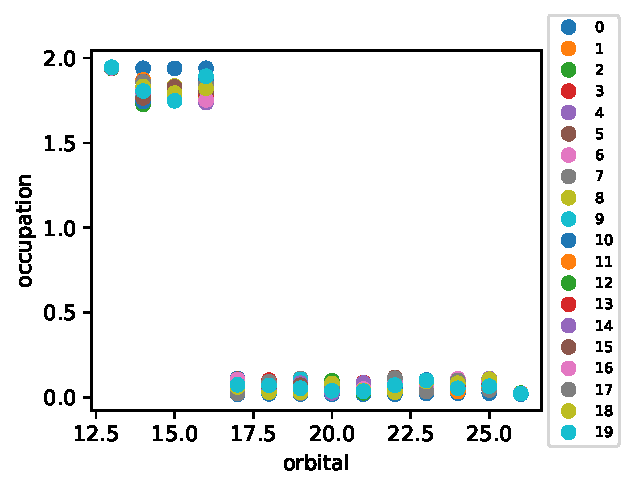
\includegraphics[width=0.5\textwidth]{images/dmc_lowen_descriptors.pdf}
\label{fig:descriptors}
\caption{Occupation of orbitals for different samples. Each color is a sample, orbital index varies along the x-axis.}
\end{figure}

The correlation matrix of the descriptors shows how the energy is correlated with the orbital occupations (Fig \ref{fig:descriptors_corrmat}).
The correlation samples include both the values and derivatives of the energies and occupations.
Since there is a constant term in the model, the mean of the energies was subtracted off (but not of the derivatives).
As we should expect, the energy is negatively correlated with the valence occupations, and positively correlated with the conduction occupations.

\begin{figure}[h!]
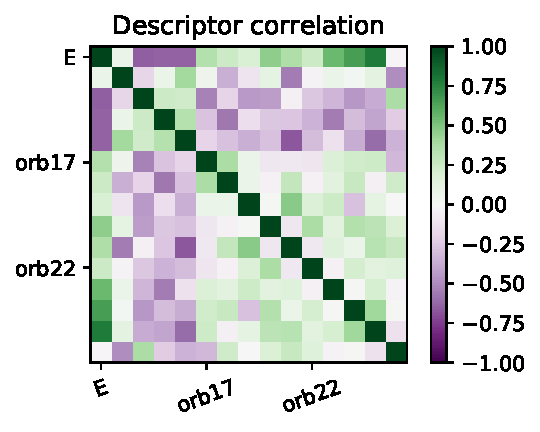
\includegraphics[width=0.5\textwidth]{images/dmc_lowen_corrmat.pdf}
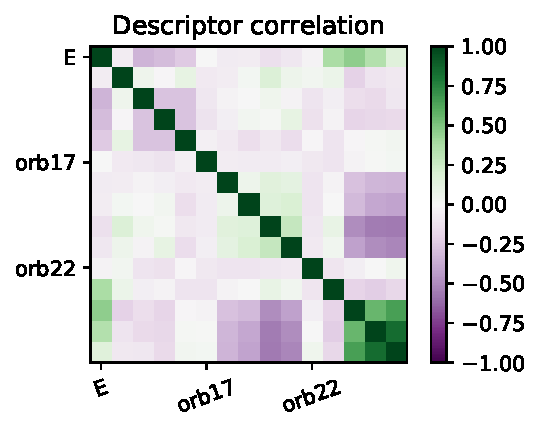
\includegraphics[width=0.5\textwidth]{images/dmc_allderivs_lowen_corrmat.pdf}
\label{fig:descriptors_corrmat}
\caption{
Left: The correlation matrix (DMC) of the energies and orbital occupations (not including derivatives). 
Right: The correlation matrix (DMC) of the energies and orbital occupations, including derivatives.}
\end{figure}

\subsection{Fitting a model}

The model is fit by linear regression.

\begin{figure}[h!]
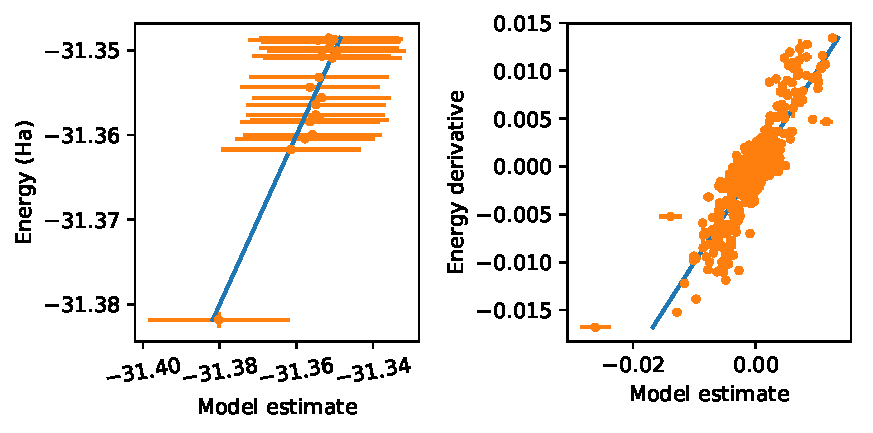
\includegraphics[width=0.65\textwidth]{images/dmc_allderivs_lowen_model.pdf}
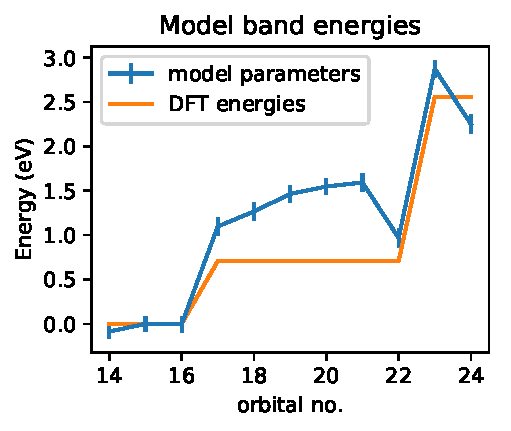
\includegraphics[width=0.35\textwidth]{images/dmc_allderivs_lowen_model_bands.pdf}
\label{fig:model_fit}
\caption{Model fit with derivatives. 
Left: Plot of data vs model prediction. 
Right: The orbital energies of the model, corresponding to shifted DFT energies.}
\end{figure}

  
  




\end{document}
